\documentclass[a4paper,11pt]{article}
\usepackage[utf8]{inputenc}
\usepackage[T1]{fontenc}
\usepackage[french]{babel}
\usepackage[right=2.5cm, left=2.5cm, bottom=4cm, top=3cm]{geometry}
\usepackage{textcomp}
\usepackage{graphicx}
\usepackage{mathtools,amssymb,amsthm}
\usepackage{lmodern}
\usepackage{multirow}
\usepackage{array}
\usepackage{longtable}

\title{\vspace{13em}{\huge Rapport Final}}
\author{Edouard Fouassier - Maxime Gonthier - Benjamin Guillot\\
		Laureline Martin - Rémi Navarro - Lydia Rodrigez de la Nava
		\vspace{2em}\\
		Algorithme Génétique
		\vspace{2em}}

\begin{document}
	
	\pagenumbering{gobble}\clearpage
	\maketitle\vspace{13em}
\newpage
\tableofcontents
\newpage\clearpage\pagenumbering{arabic}

	\section{Introduction}
		Dans le cadre du module IN608 du dernier semestre de notre Licence Informatique à l’UVSQ, nous avons eu l’occasion de réaliser un projet sous la direction de Mme Leila Kloul.\\
		Nous avons choisi, parmi les sujets proposés, le sujet Algorithme Génétique car c’est un sujet qui demande à la fois des connaissances basiques en biologie et des connaissances plus poussées en algorithmique, ce qui nous a beaucoup plu.
		De plus c’est un sujet qui demande de transformer en programmation des méthodes biologiques, ce qui est un défi intéressant.\\
		
		Notre projet consiste à créer un logiciel permettant à un utilisateur de résoudre un problème d’optimisation grâce à un Algorithme Génétique.\\
		Mais tout d’abord, qu’est-ce qu’un Algorithme Génétique ?\\
		C’est en 1960 que John Holland, professeur à l’Université du Michigan, commence à étudier la création d’un algorithme qui s’inspire de la théorie de l’évolution de Darwin, et qui résoudrait des problèmes d’optimisation de manière efficace.
		Le premier livre faisant part du sujet, Adaptation in Natural and Artificial System, fut publié en 1975 mais l’algorithme ne sera rendu populaire qu’en 1989, lors de la publication de Genetic Algorithms in Search, Optimization, and Machine Learning par David Goldberg.
		Un algorithme génétique, ou AG, s’inspire de la nature en se basant sur la sélection naturelle, c’est-à-dire qu’une population est composée d’individus qui ont plus ou moins de chance d’être sélectionnés pour se reproduire dans le but de créer de nouveaux individus de la prochaine génération.
		De cette façon, au bout d’un certain nombre d’itérations de cette sélection, les individus les plus forts seront les résultats les plus adaptés au problème.\\
		Les AG sont entre autres utilisés dans le domaine de la génétique, pour résoudre une fonction mathématique, pour optimiser un portefeuille ou encore dans le domaine de l’apprentissage.\\
		L’objectif de notre projet est donc d’implémenter un tel algorithme pour permettre à un utilisateur d’entrer des données à son problème et d’obtenir les résultats de ce dernier en sortie.
		Pour cela, il fallait tout d’abord une interface dans laquelle l’utilisateur entre une par une ses données, ou entre un fichier où sont déjà enregistrées ses données.
		Il fallait aussi que l’algorithme soit générique pour pouvoir prendre en charge un maximum de problèmes.\\
		Le logiciel se veut ergonomique avec une interface intuitive, qui ne nécessite pas de prérequis autre qu’une ou deux fonctions à optimiser.
		Pour le reste des données, l’utilisateur sera guidé dans le manuel d’utilisation pour utiliser les données les plus efficaces au fonctionnement de l’AG.\\
		Une itération de l’algorithme génétique comporte plusieurs étapes : l’évaluation des individus : à chaque individu est attribué un score par rapport à la ou les fonctions d’évaluation donnée(s) par l’utilisateur, ensuite la sélection des individus qui pourront créer de nouveaux individus, puis le croisement de deux individus sélectionnés, ou crossover, qui auront un probabilité plus ou moins élevée d’être mutés.\\
		Nous avons choisi d’implémenter notre logiciel dans le langage de programmation C++ car c’est un langage hybride. Il était nécessaire d’avoir une partie procédurale pour effectuer les calculs sur les individus, pour les tests et pour la gestion des fichiers d’entrées / de sortie. Il fallait aussi une partie objet pour l’implémentation des individus et de la population.
	
	\section{Explication de l’architecture}
		\underline{Organigramme :}\\
		\centerline{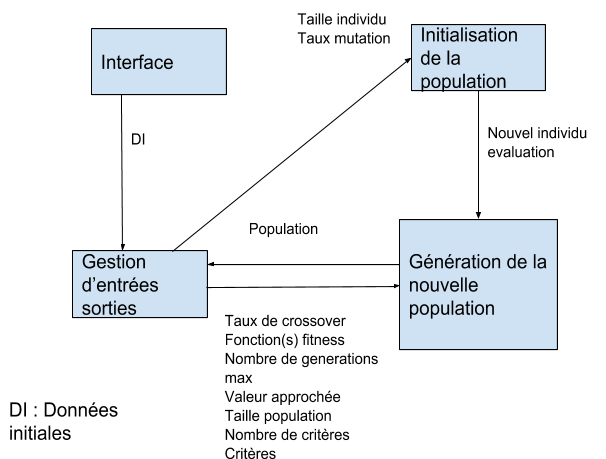
\includegraphics[scale = 0.5]{OrganigrammeV9.png}}\\
		
		Notre logiciel est organisé en 4 modules :\\
		\begin{itemize}
			\item L’initialisation de la population
			\item La génération d’une nouvelle population
			\item La gestion des fichiers d’entrées et sorties
			\item L’interface\\
		\end{itemize}
		Le module Interface est implémenté avec le logiciel Qt et est par conséquent une classe.\\
		Les modules d’initialisation de la population et de génération de nouvelle population sont toutes deux des classes qui implémentent respectivement les individus et une population.\\
		Le choix d’en faire des classes a été motivé par les possibilité de manipulation offertes de ces des notions en temps qu’objet.
		Un Individu et une Population étant composé de plusieurs éléments, l’utilisation de classe nous a permis d’en faire des attributs de ces classes tel que l’ensemble de chromosome pour un Individu ou l’ensemble d’individu pour une population.\\\\
		
		Le module de gestion d’entrées sorties est quant à lui le seul module procédural du projet. Ce module contient de la lecture, de l’écriture et des calculs. Aucuns attributs n'étant nécessaires dans ce module, en faire un objet n'aurait pas été logique. Une gestion procédurale de la gestion des entrées sorties était donc tout indiqué. \\
		
		\subsection{Initialisation de la population}
			Un individu est dans notre logiciel implémenté comme un tableau de gènes qui peuvent prendre comme valeur 0 ou 1.
			Ce tableau est de la taille entrée par l’utilisateur avec une case ajoutée au début du tableau pour le signe (0 est positif, 1 est négatif).
			Chaque individu a aussi son score et son rang, en fonction du critère.\\
			La classe Individu a aussi trois éléments statiques : probabilité de mutation, taille de l’individu et nombre de critères.
			Ceux-ci sont récupérés grâce au module de gestion d’entrée et sortie qui envoie un tableau de trois cases contenant ces éléments.\\
			L’individu peut être initialisé à 0 ou bien peut être créé de manière aléatoire. Cette dernière option est notamment utilisée pour créer la toute première population de l’AG.\\
			C’est dans ce module qu’un individu est évalué.
			En effet, il est d’abord décodé puis entré dans la fonction fitness pour obtenir le score.
			Une fois l’individu créé ou évalué, il est envoyé au module de Génération d’une population.
		
		\subsection{Génération de la nouvelle population}
		
			Le rôle de ce module est de générer une population.
			Une population est un vecteur d’individus, initialisé en fonction des données envoyées par le module de gestion d’entrée et sortie (cf organigramme page 2).\\
			Ce module effectue de plus les tests qui permettent de savoir s’il faut continuer ou pas l’itération de l’AG.
			Il teste notamment si le nombre de génération à créer a été atteint ou si les résultats convergent, auxquels cas l’AG s’arrête et le module de gestion d’entrée et sortie écrit le fichier de résultats final.\\
			De plus, c’est dans ce module qu’on retrouve les opérateurs principaux de l’algorithme génétique.
			En effet, on y trouve la sélection pour laquelle on évalue les individus puis on les trie par rapport à leur score afin d’effectuer une sélection par rang.
			On y trouve aussi le crossover qui se sert de sélection pour choisir deux individus et les croiser, puis ajouter les nouveaux individus dans la population.
			Le choix de la technique utilisée pour chacun de ces outils seront expliqués plus tard dans le rapport.\\
			Avec tous ces opérateurs, on peut donc générer une nouvelle population.\\
			Une fois que celle-ci est pleine, elle est évaluée puis envoyée au module de gestion d’entrée et de sortie pour écrire les scores de chaque individu et les statistiques de la population.\\

			Afin de réaliser notre application, nous avons été confrontés à plusieurs contraintes et choix. Nous avons dû par exemple choisir entre plusieurs algorithmes de sélection ou plusieurs algorithmes de crossover.\\
			Pour la sélection des individus, plusieurs choix s’offraient à nous. Parmi eux se trouvaient la sélection par roulette, la sélection élitiste, la sélection par tournoi et la sélection uniforme.
			La sélection élitiste choisit uniquement les meilleurs individus, donc le hasard n’est pas du tout pris en compte, ce qui ne correspondait pas à notre objectif d’inclure une part de hasard comme la sélection naturelle.
			La sélection par tournoi confronte les individus deux à deux et choisit le meilleur score.
			Cette sélection inclut une part de hasard mais les scores les plus faibles seront toujours absents de la sélection.
			La sélection uniforme est complètement aléatoire et ne permet donc pas d’optimiser nos résultats.
			Ainsi nous avons choisi la sélection par rang, qui est une forme de sélection par roulette qui inclut une part de hasard tout en sélectionnant majoritairement les meilleurs individus.\\
			Pour le crossover nous avions le choix entre un croisement en un point ou multipoint.
			Nous avons choisi le crossover à un seul point car il permet d’éviter une convergence prématurée. De plus cette technique est plus proche de la réalité biologique.

		\subsection{Gestion d'entrée sortie}
			Le module gestion d’entrée et sortie se charge de tout ce qui touche à l’écriture ou la lecture dans un fichier.\\
			On a vu précédemment que le module de gestion d’entrée et sortie recevait du module interface soit les données une à une soit un fichier de données.
			Dans le premier cas, le module se charge de les écrire dans un nouveau fichier.
			Dans le deuxième cas, on parcourt le fichier pour vérifier que toutes les données sont cohérentes. Dans les deux cas, le module vérifie que la fonction fitness est parsable.
			Pour qu’une fonction soit parsable elle doit être correctement parenthésée, ne pas avoir de division par zéro, avoir correctement orthographié les fonctions mathématiques et n’avoir qu’une seule variable nommée obligatoirement ‘x’.\\
			Une fois toutes ces données vérifiées, le module se charge d’envoyer toutes les données nécessaires au fonctionnement du module d’initialisation de la population et au module de génération d’une population. 
			Les données en questions seront utilisées dans les constructeurs des deux classes et seront par la suite exploités dans ces modules.A chaque itération de l’algorithme génétique, le module reçoit de Génération d’une population la population qui vient d’être créée.
			Il prend celle-ci et écrit le score de chaque individu dans un fichier.\\
			Le module calcule ensuite les statistiques d’une population, c’est-à-dire qu’il écrit le score du meilleur individu, du moins bon et fait un moyenne pondérée de toute la population.\\
			En s’aidant des statistiques précédemment obtenues, à la fin du programme, le module va écrire dans le(s) format(s) souhaité(s) par l’utilisateur le fichier final qui fait une synthèse du déroulement de l’algorithme et aussi le résultat à son problème.
		
		\subsection{Interface}
			Le module interface est le module qui s’occupe de la création et de l’affichage des champs de saisie. nous avons choisi d'utiliser la librairie Qt car elle est simple à utiliser, générique et donne beaucoup de liberté quand à son utilisation.\\	
			L’interface laisse le choix à l’utilisateur d’entrer ses données une par une, ou bien d’entrer le chemin  d’un fichier où celles-ci se trouvent.
			Le module vérifie que les données écrites sont correctes directement dans l’interface dans le premier cas.
			On étudiera en détail dans la partie Description du fonctionnement quelles données sont nécessaires.\\

			Le module présente également à l’utilisateur plusieurs boutons.
			Tout d’abord le bouton Aide qui ouvrira le manuel d’utilisation au cas où l’utilisateur a un doute sur l’utilisation de l’interface.\\
			Le bouton Lancer lance l’algorithme génétique si toutes les données sont correctes.
			Autrement l’utilisateur est prévenu de ses erreurs et retourne sur l’interface pour les corriger.\\
			Le bouton Arrêter arrête l’itération de l’AG lancé, mais enregistre les données et fournit le fichier de sortie malgré tout.\\
			Le bouton Quitter quant à lui arrête l’AG sans rien enregistrer.\\
			Dans le cas où l’utilisateur a entré ses données dans les champs de saisie de l’interface, celles-ci sont envoyées au module d’entrée et sortie pour qu’elles soient enregistrées dans un fichier.
			Dans le cas où l’utilisateur a entré directement un fichier de données, le nom de ce dernier est envoyé au module d’entrée et sortie qui se chargera de vérifier la cohérence des données.\\
	
	\section{Description du fonctionnement}
		\subsection{Description et Exemple d’utilisation}
			Pour décrire le fonctionnement de notre programme, nous allons nous baser sur un exemple simple et concret.
			On souhaite maximiser la fonction f(x) = x sur l'intervalle [-31; 31].
			Pour cela, on choisit une population de 10 individus, et un nombre maximum de génération de 30.
			On entre dans l’interface graphique les données suivantes :\\
				\begin{itemize}
					\item	Une ou deux fonction(s) fitness (c’est-à-dire la fonction nécessaire à l’évaluation d’un individu). 
							Il choisit ensuite s’il veut maximiser, minimiser, ou s’approcher d’une valeur. 
							Pour notre exemple, on a une seule fonction fitness qui est f(x) = x. On indique que c’est une fonction à maximiser.

					\item 	Le nombre maximal de génération, compris entre 2 et 1000 plus le nombre de générations sera elevé plus les resultats seront exacts. 
				
							Pour notre exemple, on indique 30 générations au maximum.		
					\item	La taille des individus (en nombre de bits), compris entre 1 et 32 plus les individus seront grands, plus les solutions pourront être élevé.
							On rappelle qu’un individu est codé en binaire, donc la valeur maximum que peut prendre un individu est 2\^{}(le nombre de bits)-1.
							Dans notre exemple, on choisit 10 individus de taille 5, puisque 2\^{}5-1 = 31. 
					\item	La taille des populations, compris entre 1 et 100 plus il y a d'individus dans une population, plus les solutions seront diversifiées.
							Pour notre exemple, la taille de la population sera de 10 individus.
					\item	Le taux de crossover, compris entre 0 et 1. C'est la probabilité que deux individus en génèrent deux nouveaux.
							Ici le taux de crossover sera de 0,5 pour que les individus parents en enfants aient les mêmes chances d'être introduit dans la nouvelle population.
					\item	Le taux de mutation, compris entre 0 et 1 c'est la probabilité qu'un bit soit changé aléatoirement.

							Dans le cas présent, nous souhaitons une faible probabilité de mutation pour éviter une convergence prématurée, la probabilité de mutation est donc de 0.15.
					\item	Les différents formats de sortie, il a le choix entre LaTeX, PostScript et xFig, chaque format selectionné génère un fichier.

							Dans notre exemple, on choisit uniquement la sortie LaTeX.
					\item	Le nom du fichier de sortie, c'est le nom que l'utilisateur veut donner au(x) fichier(s) qui seront généré(s).
							Le nom sera ici "exemple".\\
					\end{itemize}
			Si l’utilisateur possède déjà un fichier de données, il peut  sélectionner un fichier qui contient toutes les informations nécessaires pour démarrer le programme (décrites au-dessus).
			Les informations dans le fichier doivent être dans le bon ordre.
			Cela lui évite d’entrer les valeurs dans l’interface.\\
			Dans cette seconde option, le fichier devra impérativement respecter le format suivant :
				\begin{itemize}
					\item Taille d'un individu en nombre de bits (de 1 à 32), bit de signe non inclut.
					\item Taux de mutation (0 à 1)
					\item Taux de crossover (0 à 1)
					\item Taille de la population (2 à 100)
					\item Nombre maximum de génération (1 à 1000)
					\item Nombre de critères (1 ou 2)
					\item Première fonction fitness (voir partie 4 du manuel d'utilisation page xx)
					\item Critère de la première fonction fitness (1=maximisation 2=minimisation 3=utilisation d'une valeur approchée)
					\item Valeur approchée de la première fonction fitness (-1000 à 1000, inutile si critère différent de 3)
					\item Deuxième fonction fitness (voir partie 4 du manuel d'utilisation page xx, inutile si il n'y a qu'un critère)
					\item Critère de la deuxième fonction fitness (1=maximisation 2=minimisation 3=utilisation d'une valeur approchée, inutile si il n'y a qu'un critère)
					\item Valeur approchée de la deuxième fonction fitness (-1000 à 1000, inutile si critère différent de 3, inutile si il n'y a qu'un critère)
					\item Les formats de fichier de sortie du programme sous forme de 3 chiffres, 1 ou 0, si on veux ou non une sortie de ce format (latex postscript xfig)
				\end{itemize}
			Les valeurs inutiles ne génèrent pas d'erreur.\\
			Des fichiers d'exemples sont fournis.\\\\
			Dès que l’utilisateur a entré toutes les valeurs ou qu’il a entré le fichier des paramètres, il peut lancer le programme en cliquant sur le bouton “Lancer”.\\
			Il peut à tout moment de l'éxécution arrêter ou quitter le programme. Le bouton “Arrêter” permettra d’arrêter le programme en sauvegardant les résultats en cours.\\
			Alors que le bouton “Quitter” permettra d’arrêter le programme sans sauvegarder les résultats en cours.\\
			Enfin, si l’utilisateur a un doute, il peut consulter le manuel d’utilisation via le bouton “Aide”.\\\\
			Voici l’interface remplie avec les valeurs de notre exemple juste avant de lancer le programme :\\
			\centerline{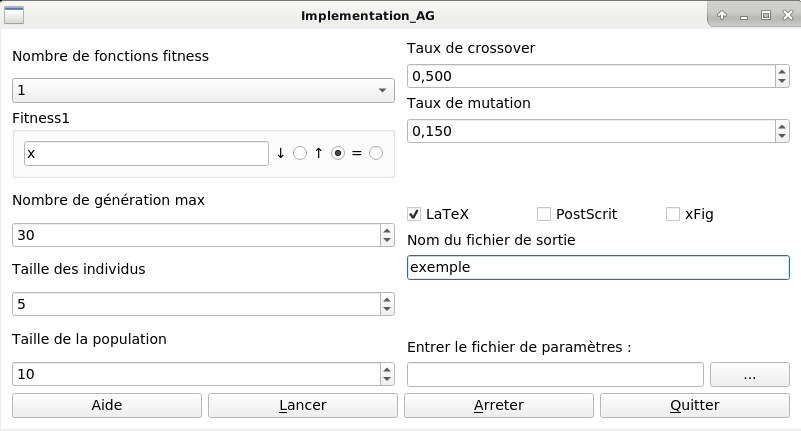
\includegraphics[scale=0.5]{Interface.png}}
			
		\subsection{Explication du fonctionnement de l’algorithme}
			Le lancement de l’algorithme se passe dans la fonction \textbf{Interface::algoGenetique}.\\
			Dans un premier temps, une génération composée d’individus aléatoires est créée à l’aide des données entrées par l’utilisateur : c’est la population initiale.\\
			Avec le même exemple que dans la partie 1, la population initiale peut être :\\
			\centerline{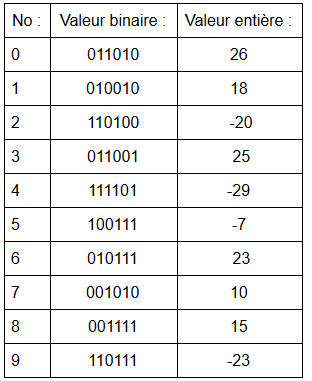
\includegraphics[scale=0.5]{ExemplePopulationInitiale.png}}
			Le bit de poid fort est le bit de signe.\\
			
			Les individus sont alors évalués dans la fonction \textbf{Population::evaluation()} qui fait appel à la fonction \textbf{Individu::evaluationIndividu(string, int)}.\\
			L’évaluation consiste à remplacer “x” dans la fonction fitness passée en argument et renvoyer un score qui est mis dans float* score[] (attribut de la classe Individu).\\
			Pour notre exemple, comme la fonction fitness est f(x) = x, le score est simplement la valeur de l’individu. Le tableau des scores ressemblera donc à : \\
			\centerline{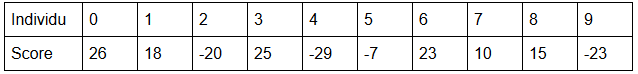
\includegraphics[scale=0.5]{Evaluation.png}}\\
			
			Toujours dans la méthode \textbf{Population::evaluation()}, les individus sont triés selon leur(s) score(s) grâce à la fonction \textbf{Population::triPopulation(int)}.
			Selon le critère sélectionné, cette méthode va faire appel à la méthode \textbf{Population::maximisation(int)} (si la fonction fitness est à maximiser), \textbf{Population::minimisation(int)} (si la fonction fitness est à minimiser) ou \textbf{Population::triValeur(int)} (si la fonction fitness doit s’approcher d’une valeur).
			Dans notre cas, la fonction fitness est à maximiser. La méthode concernée réorganise le vecteur ensemble (attribut de la classe Population) de manière à avoir les individus dans l’ordre décroissant selon leur score.
			Le vecteur ensemble est maintenant :\\
			\centerline{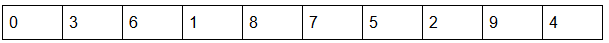
\includegraphics[scale=0.5]{VecteurTrie.png}}\\
			
			Puis dans la méthode \textbf{Population::evaluation()} un rang est attribué à chaque individu selon leur score dans int rang[] (attribut de la classe Individu).
			Pour les critères de maximisation et de minimisation, le rang se fait en une simple lecture du vecteur ensemble.
			Le rang est croissant et si deux individus ont le même score, ils auront le même rang.
			Pour le critère de valeur approchée, le rang est la différence entre le score de l’individu et la valeur à approchée.
			Dans notre exemple, le rang pour chaque individu est :\\
			\centerline{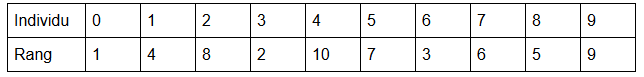
\includegraphics[scale=0.5]{RangIndividu.png}}\\
			
			Puis la méthode \textbf{Interface::algoGenetique()} boucle et teste avec la fonction \textbf{testArret()} si le nombre de génération maximum est atteint ou si les résultats convergent.
			Si l’une de ces conditions est remplie alors on arrête le programme, sinon, on crée une nouvelle population qui sélectionne des individus et les croise ou non.
			Dans ce second cas, la méthode \textbf{Population::creerGeneration(Population*)} fait appel à la méthode \textbf{Population::selectionner(int)} sur la population passée en argument.
			Cette méthode se base sur la méthode de la roulette biaisée.
			Cela signifie que les individus ayant un rang proche de 1 ont une plus grande chance d’être sélectionnés.
			Pour illustrer, on montre deux appels à la méthode \textbf{Population::selectionner(int)}. Elle renvoie les individus 0 et 6.\\

			Les deux individus sélectionnés sont ensuite passé en argument de la méthode \textbf{Population::crossover(Individu*, Individu*)}.
			Cette méthode utilise le taux de crossover.
			Soit les deux individus sont croisés et créent deux individus “enfants” qui sont ajoutés à la nouvelle population, soit les deux individus sont directement ajoutés à la nouvelle population.
			Si les deux individus sélectionnés doivent être croisé, la nouvelle population reçoit les deux nouveaux individus suivants :\\
			\centerline{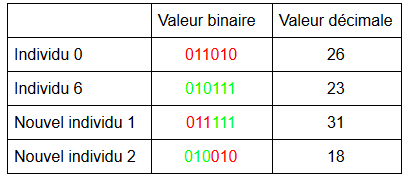
\includegraphics[scale=0.5]{Crossover.png}}
			Le bit de poid fort est le bit de signe.\\
			Le point de croisement, c’est-à-dire le point où les individus sont coupés pour être recombinés est choisi aléatoirement entre 1 et la taille des individu -1.\\
			
			Pour finir, cette nouvelle population remplace alors la population précédente. Puis elle est évaluée et on retourne au début de la boucle.\\
			
			Une fois le programme terminé, nous obtenons un fichier LaTeX, converti en PDF nous obtenons ce graphique et la solution adéquat :\\
			\centerline{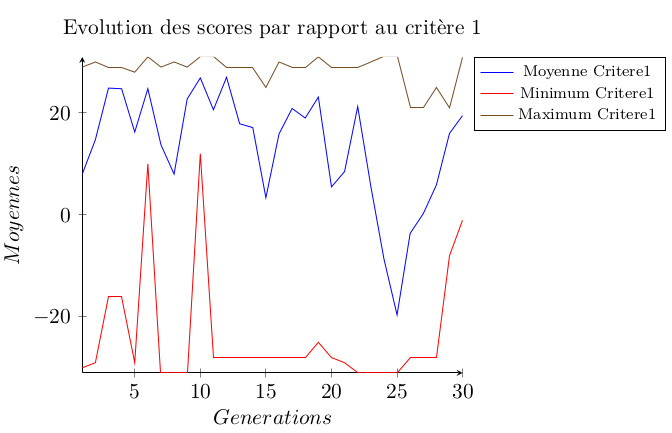
\includegraphics[scale=0.5]{Graphe.png}}\\\\
			\centerline{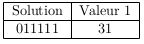
\includegraphics[scale=0.5]{Resultats.png}}\\
			
			Notre exemple de maximisation de la fonction f(x) = x, un ensemble de solutions n’est pas nécessaire, et on choisit la plus grande solution ici 31 (ce qui est le résultat attendu).
			Le graphique montre l’évolution de l’ensemble des générations.
			En lisant le tracé marron (Maximum critère 1), on remarque que le maximum a très vite été trouvé dans les premières générations.
			On peut se demander dans ce cas très simple pourquoi on utilise un algorithme génétique au lieu d’une simple exploration de toutes les possibilités.\\
			Néanmoins dans la réalité, les fonctions peuvent être bien plus complexes et sur un bien plus grand espace de recherche, auquel cas un algorithme est plus efficace qu’une recherche exhaustive puisqu’il cherche simplement à maximiser (ou minimiser) sans information autre que la fonction à optimiser.
		
		
		\section{Points délicats de la programmation}
		\subsection{Les algorithmes }
			L’objectif de la fonction \textbf{estParsable} est de tester si la fonction fitness entrée par l’utilisateur respecte les conditions que nous avons posées.\\

			La première difficulté a été le test qui détermine si la fonction donnée a une syntaxe valide (une seule variable appelée “x”, bonne écriture des fonctions mathématiques, etc.).\\
			Pour cela, la fonction lit  un à un les caractères de la fonction fitness. A chaque lettre lue, la fonction teste si les lettres suivantes forment bien une fonction mathématique valide. \\
			Il fallait donc imbriquer de nombreux \textbf{if} pour tester toutes les possibilités. La seconde difficulté a été de tester la présence de divisions par zéro. Nous avons donc écrit dans des chaînes de caractères les dénominateurs de chacune des fractions puis nous les avons évalués un à un avec le parseur.\\

			Une autre des difficultés rencontrées a été d'optimiser l'utilisation des fichiers via les fonctions tout en assurant le maintient d'une certaine ergonomie.
			Lors de l'implémentation des fonctions \textbf{ecrirePostscript} et  \textbf{ecrireXfig} écrire les fichiers postscript et xfig s’est révélé plus compliqué qu’escompté, car n’ayant pas su appréhender correctement le langage PostScript, la création du fichier .ps a été ardue et le format .fig étant un format d’image il s’est avéré difficile de créer une image .fig directement à partir des données.\\
			L’écriture des deux fichiers se fait donc grâce à une suite de commandes. Pour le fichier postscript si l'écriture du fichier en latex a été demandée par l’utilisateur, on convertit le fichier latex en fichier dvi puis en fichier postscript et on supprime ensuite le fichier dvi; si l'utilisateur n’a pas demandé le fichier en latex alors il est quand même écrit mais après les conversions permettant d’obtenir le fichier postscript, on supprime également le fichier latex.\\
			Pour le fichier xfig on génère tout d’abord un fichier gnuplot qui est ensuite converti en fichier .fig et ensuite supprimé pour ne garder que le fichier .fig.\\

			La fonction permettant de tester la convergence \textbf{testConvergence} a pour objectif de tester les valeurs moyennes des x dernières générations.\\
			Le principal problème rencontré étant que ces valeurs étaient stockées dans un fichier et qu’à chaque itération de l’algorithme une nouvelle valeur était ajoutée à la fin de ce fichier.\\
			Il a donc fallu trouver un moyen d’isoler uniquement ces valeurs afin de pouvoir les analyser ce qui nous a posé quelques difficultés. Nous avons finalement opté pour une option nous permettant de modifier le moins possible la fonction par rapport au cahier des spécifications.\\
			Nous récupérons donc uniquement le nom du fichier de statistiques en paramètres puis stockons dans un tableau de taille nombreGeneration (ce qui correspond au nombre d’itérations actuelles de l’algorithme) et récupérons les x dernière valeurs de ce tableau pour tester la convergence.\\

		\subsection{Les modifications par rapport au cahier des spécifications}
			Lors de l’implémentation, nous nous sommes rendus compte que nos choix de paramètre de fonction ou de type de fonction n’étaient pas forcément optimaux donc nous avons dû appliquer quelques changements.\\
   			Notamment, nous n’avions pas pris en compte les pointeurs dans notre raisonnement, donc plusieurs fonctions ont des pointeurs ajoutés en paramètres comme par exemple \textbf{ecrirePopulation(Population *P)}. On évite ainsi des problèmes de mémoire. \\

   			\subsubsection{Les modifications dans le module Gestion d’entrée et de sortie}
   				\begin{itemize}
   					\item Pour la fonction  \textbf{lireStat}, nous sommes passés d’un type int[3] à un type float* car c’est un tableau de float que nous devons renvoyer, puisque le minimum, le maximum et la moyenne peuvent très bien être des float.
   					Il en va de même pour la fonction  \textbf{lireScoreIndividu} qui initialement avait pour signature un int mais qui maintenant est un float* car les scores peuvent eux aussi être des nombres à virgule et dans le cas du multi-critères, il faut renvoyer deux valeurs et non une seule.

   					\item Les fonctions  \textbf{ecrireFichier} et  \textbf{ecrireLatex} prennent maintenant un nouveau paramètre : Population *P qui permet de récupérer les meilleurs individus qu’on écrit dans le fichier .tex. Le paramètre string nomFichierStats de la fonction  \textbf{ecrireFichier} a quant à lui été retiré car il n'était pas utile.
   					\item La fonction  \textbf{ecrireUnScore} a été retirée entièrement car elle était finalement inutile, la fonction  \textbf{ecrirePopulation} remplissant ce rôle.

   					\item Pour les fonctions de vérification des données ( \textbf{estString},  \textbf{estParsable} etc…) nous sommes passés d’un auto en paramètre des fonctions à un string. Le type auto ne nous permettait pas d'appeler ces fonctions avec notre interface, nous avons donc opté pour le type string qui remplit le même usage sans ce défaut.
   				\end{itemize}

   			\subsubsection{Les modifications dans le module Génération d’une population}
   				Le module de génération de la population comporte quelques modifications par rapport au cahier des spécifications.\\
   				\begin{itemize}
   					\item La première modification concerne l’attribut  \textbf{ensemble}. Initialement un tableau d’individu (individu *) cet attribut est maintenant un vecteur d’individus (vector<Individu*>). Ce choix est motivé par la plus grande intuitivité d’utilisation des vecteurs en C++ par rapport aux tableaux. De ce fait le getter getEnsemble est également modifié, renvoyant maintenant un vecteur et non un tableau.

   					\item Il y a également une légère modification sur le constructeur  \textbf{Population(string *const\& donnees)}. En effet une données est ajoutée au paramètre donnees. Cette donnée supplémentaire étant le nom du fichier de paramètre, elle nous permet de récupérer les information nécessaires à la créations d’un individu en utilisant le constructeur  \textbf{Individu(float donnees[3])}. De ce fait les individus créés par ce constructeur de Population le seront avec les données nécessaire pour allouer à la bonne tailles les attributs int* chromosome, float* score et int* rang.

   					\item La modification de la fonction  \textbf{testArret} concerne sa signature. En effet renvoyer une population comme prévu initialement n’était pas nécessaire. Utiliser un bool était plus judicieux pour interpréter le résultat de cette fonction.

   					\item La modification de la fonction  \textbf{testConvergence} concerne ses paramètres. Le fichier de statistiques du programme devait initialement toujours avoir le même nom et donc le passer en argument n’était pas nécessaire. Cependant lors de l’implémentation de l'application nous avons finalement décidé de mettre tous les fichiers relatifs à une exécution du programme dans un fichier créé spécialement pour l’occasion. Le nom de ce dossier étant entré par l’utilisateur et le nom du fichier de statistique en dépendant, il a donc fallu le passer en paramètre de la fonction.

   					\item La modification de la fonction d’évaluation de la population \textbf{evaluation} concerne sa signature. En effet renvoyer une population n’était pas utile et nous avons donc choisi de la changer pour un void pour ne pas créer de confusion.

   					\item La modification de la fonction  \textbf{triPopulation} concerne sa signature. En effet renvoyer un bool comme prévu initialement n’était pas nécessaire. De ce fait pour éviter toute confusion lors de son utilisation nous avons décidé de remplacer cette signature par un void.
					De plus, les trois fonctions  \textbf{maximisation},  \textbf{minimisation} et  \textbf{triValeur} sont un ajout par rapport au cahier des spécifications. Elles ne modifient aucunement le fonctionnement du programme tel que décrit dans le cahier des spécifications, ni celui de la fonction de tri décrite dans ce même document. Elles ont un intérêt purement esthétique et permettent de rendre le code plus lisible.

					\item Dans la fonction  \textbf{Individu* selectionner(int iCritere)}, on a ajouté un argument qui précise dans quel critère on cherche à sélectionner les individus.
					Quant à la fonction de  \textbf{crossover}, nous avons finalement trouvé qu’il n’était pas utile qu’elle renvoie une population. Nous l’avons transformée en une fonction void qui modifie directement l’objet :  \textbf{void crossover(Individu *Parent1, Individu *Parent2)}.

					\item Nous avons également du ajouter un attribut et quelques fonctions par rapport au cahier des spécifications. Ces modifications ne changent en aucun cas le fonctionnement de l’application et sont seulement dû à des oublis. En effet lors de la rédactions du cahier des spécifications nous nous sommes concentrés sur les fonctions spécifiques au bon fonctionnement de l’algorithme génétique. Notre attention étant retenue sur ce point nous avons donc oublié l’attribut  \textbf{static float valeurApprochee2}. Par conséquent nous avons donc également dû ajouter le getter et setter de cet attribut soit  \textbf{float getValeurApprochee2()} et  \textbf{void setValeurApprochee2(float val)}. Dans notre inattention lors de la relecture nous avons également oublié les getter  \textbf{int getNombreGenerationMax()} et  \textbf{int getNombreCriteres()}. Nous avons aussi dû modifier le setter pour l’attribut ensemble qui était écrit comme un getter. Dans ce cas la signature de la fonction a été modifié pour devenir  \textbf{void setEnsemble(Individu \&nouv)}.\\
				\end{itemize}

			\subsubsection{Les modifications dans le module Initialisation de la population}
				Nous avons également procédé à quelques modifications dans le module d’Initialisation de la population.\\
				\begin{itemize}
					\item Nous avons ajouté un constructeur dans la classe Individu. Il s’agit d’un constructeur de copie d’individu  \textbf{Individu(Individu I)}. Ce constructeur est utile dans la méthode  \textbf{void crossover (Individu *Parent1, Individu *Parent2)} de la classe Population dans le module Génération d’une population.

					\item Nous avons ajouté une méthode  \textbf{int décodage(int* binaire)}. Cette méthode est  utile dans la fonction bool  \textbf{evaluationIndividu(string fonctionFitness, double valeur)}. On récupère simplement le tableau chromosome de l’individu en cours et on passe ce tableau dans la fonction de décodage.\\
				\end{itemize}

			\subsubsection{Les modifications dans le module Interface}
				Il a fallu ajouter un booléen  \textbf{bool encours} permettant de savoir si le programme a été lancé. Cela change les messages affiché par les différents boutons.\\
				Nous avons aussi dû modifier la fonction  \textbf{void algoGenetique()} en  \textbf{void * algoGenetique(void * arg)} car cette fonction est lancée avec un thread.
				Nous n’avions pas pris en compte que le déroulement de l’algorithme ne permettait pas l’utilisation de l’interface et notamment du bouton d'arrêt. L’utilisation du thread laisse le processus se lequel se trouve l’interface libre .\\

			\subsubsection{Autres problèmes}
				Au début du projet nous avions aussi de gros problèmes dans nos résultats puisque généralement les valeurs convergeaient au bout de seulement quelques générations. Nous nous sommes plus tard rendus compte que le problème venait de la conversion des données de string à flottant. Nous utilisions la fonction  \textbf{stof(string)} pour convertir les strings en float, mais celle-ci renvoyait une valeur entière, or pour une probabilité de crossover de 0,8 on avait 0 donc jamais de crossover, d’où la convergence prématurée.\\
				Pour évité cela nous avons convertie les string en QString car cet objet a de nombreuses méthodes notamment de conversion. Nous utilisons donc la fonctions  \textbf{toFloat()} du QString afin de récupérer la valeur.\\

		
	\section{Conclusion technique}
		On a vu précédemment les utilisations de notre logiciel final. Nous allons maintenant parler de ses défauts et de ses possibles améliorations.\\
		Son défaut principal est qu’il n’est pas aussi générique que nous l’aurions voulu. En effet, le logiciel ne permet à l’utilisateur que d’entrer des fonctions d’adaptation qui n’ont qu’une seule variable. De ce fait, le logiciel n’est utile que dans le cas où l’on veut observer l’évolution d’une fonction à une variable.\\
		Une solution à ce problème est de repenser le codage d’un individu. Disons par exemple qu’on cherche à trouver le plus court chemin entre 5 points. Il faudrait dans ce cas un individu dans lequel 5 points sont concaténés et où le crossover se ferait donc entre ces points. Ceci est seulement un exemple, le choix est vaste quant au codage d’un individu, mais c’est un codage qui permet de trouver des solutions à de nombreux problèmes. On peut, par exemple, créer de la musique, où chaque bloc d’un individu serait une note.  Nous pensons donc que le manque de généricité du programme pourrait être résolu en revoyant le codage d’un individu. Cette information n’est malheureusement pas ressortie dans la plupart de nos recherches sur le sujet, donc nous ne l’avons pas prise en compte lors de notre réflexion.\\
		La gestion de fonctions fitness à plusieurs variables aurait également pu permettre de rendre l'algorithme plus générique, cependant nous ne nous en étions pas rendu compte non plus lors de nos recherches.\\
		En termes d’efficacité, notre programme n’est pas parfait. Nous avons été surtout freinés par la mémoire.\\
		Par exemple, le programme serait plus efficace si la taille de la population était plus élevée. Il en va de même pour l’individu : la première amélioration de l’individu serait de ne plus limiter un gène à 0 ou 1, puisqu’ils sont implémentés comme entiers, mais de laisser choisir à l’utilisateur la taille maximum d’un gène. Ainsi, nous n’utiliserions pas 4 octets en mémoire pour un seul bit.
		Le code aussi pourrait être facilement amélioré. Par exemple, on pourrait faire plutôt un tri rapide dans la fonction de tri de la population qui sert à l’évaluation des individus. La complexité de l’algorithme serait donc moindre. Cependant d’autres fonctions plus délicates et fondamentales requéraient notre attention et nous avons décidé de ne pas effectuer cette modification qui n'était pas indispensable au bon fonctionnement de l’application.\\
		De plus, le code de la fonction estParsable est très volumineux (+ de 100 lignes) cela aurait pu être réduit en divisant la fonction par exemple où en effectuant les tests de manière plus concise.\\
		De la même façon, la lecture du fichier de statistiques dans le test de convergence peut également être améliorée afin de ne lire que les statistiques voulues et non pas tout le fichier.\\
		Pour l'écriture des fichiers .ps et .fig, il aurait sûrement été plus optimisé de ne pas avoir a passer par des lignes de commandes. Cependant nous n’avons pas réussi autrement.\\

	\section{Conclusion sur l'organisation}
		En termes d’organisation, nous avons mis en place deux rendez-vous par semaines pendant lesquels le groupe entier était présent.\\
		Le premier était prévu tous les mercredis, juste après notre entrevue avec Mme Kloul, pendant lequel nous nous répartissions les tâches et travaillons sur les remarques faites précédemment par la professeure.\\
		Nous nous retrouvions ensuite le mardi suivant pour mettre en commun toutes nos recherches et nous mettre d’accord sur nos choix pour notre projet selon le planning, et sur notre présentation du lendemain. Le reste du temps nous restions en contact via un groupe de messagerie, nous partagions nos recherches sur Google Document et sur GitHub. Lors de l’implémentation, nous avons séparé le groupe en binôme, chacun était chargé d’un module, tout en restant vigilant des autres modules.\\
		Malgré cette organisation, il y a eu des semaines pour lesquelles nous avions sous-estimé la complexité de certaines tâches, et pendant lesquelles nos réunions ne servaient non plus à rassembler les informations mais à les rechercher. Ces changements de dernières minutes nous ont poussé à nous diviser pour effectuer les recherches. Ce qui a pris de notre temps pour nous mettre d’accord et prendre des décisions.\\
		Cela a conduit à des réunions où tout le monde n’était plus concentré sur le même problème, mais plutôt sur plusieurs, ce qui a conduit à un certain manque de communication puisque tout le monde n’était pas attentif lorsqu’une décision était prise.\\
 		Il est possible que notre manque de recherches et les incohérences prennent leurs sources dans ce problème-là.\\
		Nous sommes conscients des faiblesses dans notre projet mais sortons grandis de l’expérience. Nous savons que les erreurs qui ont été faites ne seront plus reproduites dans nos futurs projets à chacun, nous avons appris beaucoup en terme d’organisation et l’importance d’une bonne cohésion de groupe.\\ 
		Chacun de nous a découvert quels sont ses points forts et ses points faibles, et nous ferons de notre mieux pour travailler sur nos points faibles et d’exploiter au mieux nos points forts. Ce projet nous a aussi appris l’importance de travailler de manière suffisamment intelligible pour que tous les membres du groupe comprennent une notion ou un morceau de code.\\

\end{document}
